% !TeX root = RJwrapper.tex
\title{Regularized Transformation Models: The \pkg{tramnet} Package}
\author{by Lucas Kook and Torsten Hothorn}

\maketitle

\abstract{
  The \CRANpkg{tramnet} package implements regularized linear 
  transformation models by combining the flexible class of transformation
  models from \CRANpkg{tram} with constrained convex optimization implemented in \CRANpkg{CVXR}.
  Regularized transformation models unify many existing and novel regularized regression
  models under one theoretical and computational framework.
  Regularization strategies implemented for transformation models in \pkg{tramnet} 
  include the Lasso, ridge regression, and the elastic net and
  follow the parameterization in \CRANpkg{glmnet}. Several functionalities
  for optimizing the hyperparameters, including model-based optimization based on
  the \CRANpkg{mlrMBO} package, are implemented. A multitude of \code{S3} methods
  is deployed for visualization, handling, and simulation purposes. This work
  aims at illustrating all facets of \pkg{tramnet} in realistic settings and comparing
  regularized transformation models with existing implementations of similar models.
}

%%%%%%%%%%%%%%%%%%%%%%%%%%%%%%%%%%%%%%%%%%%%%%%%%%%%%%%%%%%%%%%%%%%%%%%%%%%%%%%%
\section{Introduction}
%-------------------------------------------------------------------------------

A plethora of \textsf{R} packages exists to estimate generalized linear regression
models via penalized maximum likelihood, such as \CRANpkg{penalized}
\citep{penalizedpaper} and \pkg{glmnet} \citep{glmnetpaper}. Both packages come
with an extension to fit a penalized form of the Cox proportional hazard model.
The \pkg{tramnet} package aims at unifying the above-mentioned and several
novel models using the theoretical and computational framework of
transformation models. Novel models in this class include Continuous Outcome
Logistic Regression (COLR), as introduced by \citet{COLRpaper} and Box-Cox type
regression models with a transformed conditionally normal response \citep{boxcox,
pkg:tram}. 

The disciplined convex optimization package \pkg{CVXR} \citep{CVXRpaper} is
applied to solve the constrained convex optimization problems that arise
when fitting regularized transformation models.  Transformation models are
introduced in Section~\nameref{subsec:tram}. For a more theoretical treatise, we
refer to \citet{ctmpaper, mltpaper, mltjss}.  Convex optimization and domain-specific 
languages are briefly discussed in Section~\nameref{subsec:CVXR},
followed by a treatment of model-based optimization for hyperparameter
tuning (Section~\nameref{subsec:mbo}).

\subsection{Transformation models} \label{subsec:tram}

In stark contrast to penalized generalized linear models, regularized
transformation models aim at estimating the response's whole conditional distribution
instead of focusing on a single moment, \eg the conditional mean.
This conditional distribution function of a response $\rY$ is decomposed into an
\textit{a priori} chosen absolute continuous and log-concave error distribution
$F$ and a conditional transformation function $\h(\ry \given \rx, \rs)$ that depends
on the measured covariates $\rx$ and stratum variables $\rs$ and is monotone
increasing in $\ry$.
Although the model class is more flexible, 
packages \pkg{tram} and \pkg{tramnet} focus on stratified linear transformation models of the form

\begin{align} \label{fm:trafo}
	\Prb\left(\rY \le \ry \given \rX = \rx, \rS = \rs \right) =
	F\left(\h(\ry \given \rs, \rx)\right) = F\left(\h(\ry \given \rs) -
	\rx^\top\shiftparm\right).
\end{align}
Here, the baseline transformation is allowed to vary with stratum variables $\rs$,
while covariate effects $\shiftparm$ are restricted to be shifts common to all
baseline transformations $\h(\ry \given \rs)$.

In order for the model to represent a valid cumulative distribution function,
$F\left(\h(\ry \given \rs, \rx)\right)$ has to be monotone increasing in $\ry$, and thus,
in $\h$ for all possible strata $\rs$ and all possible configurations of the
covariates $\rx$. To ensure monotonicity, $\h$ is parameterized in terms of a basis
expansion using Bernstein polynomials as implemented in the \CRANpkg{basefun}
package \citep{mltjss}. Hence, $\h$ is of the form

\begin{align*}
	\h(\ry) = \bern{p}(\ry)^\top \parm,
\end{align*}
where $\bern{p}(\ry)$ denotes the vector of basis functions in $\ry$ of order $p$
and $\parm$ are the coefficients for each basis function. Conveniently,
$\bern{p}(\ry)^\top \parm$ is monotone increasing in $\ry$ as long as

\begin{align} \label{eq:const}
\begin{array}{ll}
\eparm_i \leq \eparm_{i+1}, & i = 0, \dots, p - 1
\end{array}
\end{align}
holds. For the concrete parameterization of stratified linear transformation
models, the reader is referred to \citet{pkg:tram}.

Many contemporary models can be understood as linear transformation models,
such as the normal linear regression model, logistic regression for binary,
ordered, and continuous responses, as well as exponential, Weibull and Rayleigh
regression, and the Cox model in survival analysis. Thus, by appropriately choosing
and parameterizing $F$ and $\h$, one can understand all those models in the same
maximum likelihood-based framework. One can formulate the corresponding likelihood
contributions not only for exact observations but under any form of random 
censoring and truncation for continuous and count or ordered categorical
responses.

Given a univariate response $\rY$ and a set of covariates $\rX = \rx$ and strata
$\rS = \rs$, one can specify the following cumulative distribution function and 
density valid for any linear transformation model:

\begin{align*}
  \begin{aligned}
  	\pYx(\ry \given \rs, \rx) &= F\left(\h(\ry \mid \rs) - \rx^\top \shiftparm \right), \\
  	\dYx(\ry \given \rs, \rx) &= F'\left(\h(\ry \mid \rs) - \rx^\top \shiftparm \right)
  	\cdot \h'(\ry \mid \rs).
  \end{aligned}
\end{align*}
From here, the log-likelihood contributions for exact, right, left, and interval-censored 
responses can be derived as

\begin{align*}
  \begin{aligned}
  	\ell(\parm,\shiftparm;\ry_i, \rs_i, \rx_i) &=
  	\left\{
  	\begin{array}{lll}
  	  \log\left(F'\left(\h\left(\ry_i \mid \rs_i \right) - \rx_i^\top \shiftparm
  	  \right)\right) + \log\left(\h'(\ry_i \mid \rs_i)\right) & \ry_i & \text{exact}\\
  	  \log\left(F\left(\h(\bar{\ry} \mid \rs_i) - \rx_i^\top \shiftparm\right)
  	  \right) & \ry_i  \in (-\infty, \bar{y}] & \text{left} \\
  	   \log\left(1 -
  	  F\left(\h(\ubar{\ry} \mid \rs_i) - \rx_i^\top \shiftparm\right)\right) &
  	  \ry_i \in (\ubar{\ry}, \infty) & \text{right} \\
  	  \log\left(F\left(\h(\bar{\ry} \mid \rs_i) - \rx_i^\top \shiftparm\right) -
  	  F\left(\h(\ubar{\ry} \mid \rs_i) - \rx_i^\top \shiftparm\right)\right) &
  	  \ry_i \in (\ubar{\ry}, \bar{\ry}] & \text{interval}.  \\
  	\end{array}
  	\right.
  \end{aligned}
\end{align*}
The joint log-likelihood of several observations $\{(\ry_i, \rx_i, \rs_i)\}_{i=1}^n$ is obtained
by summing over the individual log-likelihood contributions $\ell_i$ under the
assumption that the individual samples are independent and identically
distributed, the case exclusively dealt with by \pkg{tramnet}.

\subsection{Regularization} \label{regul}

The aim of \pkg{tramnet} is to enable the estimation of regularized stratified
linear transformation models. This is achieved by optimizing a penalized
form of the log-likelihood introduced in the last section. The penalized
log-likelihood,

\begin{align*}
  \pll = \ull - \llpen,
\end{align*}
consists of the unpenalized log-likelihood and an additional penalty term. Note
that only the shift parameters $\shiftparm$ are penalized, whereas the coefficients
for the baseline transformation $\parm$ remain unpenalized.
The parameterization of the penalty is chosen to be the same as in \pkg{glmnet},
consisting of a global penalization parameter $\lambda$, and a mixing parameter
$\alpha$ controlling the amount of $L_1$ compared to $L_2$ penalization.

The two penalties and any combination thereof have unique properties and may be useful
under different circumstances. A pure $L_1$ penalty was first introduced by \citet{lasso1996}
in an OLS framework and was dubbed the Lasso (Least Absolute
Shrinkage and Selection Operator) due to its property of shrinking
regression coefficients exactly to 0 for large enough $\lambda$. A pure Lasso
penalty can be obtained in a regularized transformation model by specifying
$\alpha = 1$. Applying an $L_2$ penalty in an OLS problem was introduced more than
five decades earlier by \citet{tikhonov1943stability} and later termed ridge
regression \citep{hoerl1970ridge}.
In contrast to Lasso, ridge regression leads to shrunken regression coefficients
but does not perform automatic variable selection. \citet{zou2005regularization}
picked up on both approaches, discussed their advantages, disadvantages, and
overall characteristics and combined them into the elastic net penalty,
a convex combination of an $L_1$ and $L_2$ penalty controlled by the mixing
parameter $\alpha$.
Some of these properties will be illustrated for different models and a real-world
data set in Sections~\nameref{subsec:modelclasses} and \nameref{sec:tuning}.

\subsection{Constrained convex optimization} \label{subsec:CVXR}

Special algorithms were developed to optimize regularized objective functions,
most prominently the LARS and LARS-EN algorithm \citep{efron2004} and variants
thereof for the penalized Cox model \citep{penalizedpaper}. However, the aim of
\pkg{tramnet} is to solve the objective functions arising in regularized transformation
models in a single computational framework.
Due to the log-concavity of all choices for $F$ in this package and $\h(\ry\given\rx,\rs)$ being
monotone increasing in $\ry$, the resulting log-likelihood contributions for any
form of censoring and truncation are concave and can thus be solved by constrained
convex optimization.

The fairly recent development of \pkg{CVXR} allows the specification of constrained
convex optimization problems in terms of a domain-specific language, yielding
an intuitive and highly flexible framework for constrained optimization. Because
checking the convexity of an arbitrarily complex expression is extremely hard,
\pkg{CVXR} makes use of a library of smaller expressions, called atoms, with known
monotonicity and curvature and tries to decompose the objective at hand using a
set of rules from disciplined convex optimization \citep[DCP,][]{DCPpaper}. Thus, a
complex expression's curvature can be more easily determined.

More formally, convex optimization aims at solving a problem of the form

\begin{align*}
  \begin{array}{ll}
  	\underset{\parm}{\mbox{minimize}} & g(\parm) \\
  	\mbox{subject to} & g_i(\parm) \leq 0, \; i = 1, \dots, K, \\
  	& \mA\parm = \bvec,
  \end{array}
\end{align*}
where $\parm \in \mathbb{R}^p$ is the parameter vector, $g(\parm)$ is the objective
function to be optimized, $g_i(\parm)$ specify the inequality constraints, and
$\mA \in \mathbb{R}^{n \times p}$ and $\bvec \in \mathbb{R}^p$ parameterize any
equality constraints on $\parm$. Importantly, the objective function and all
inequality constraint functions are convex \citep{boyd2004convex}.

The likelihood $\sum_i \ell(\parm, \shiftparm; \ry_i, \rs_i, \rx_i)$ for
transformation models of the form (\ref{fm:trafo}) are convex for error
distributions with log-concave density because log-convexity
of $-{F'}$ ensures the existence and uniqueness of the most likely transformation
$\hat\h$ and the convexity of $-\ell(\h; \ry, \rx)$.
Because the penalty term is convex in $\shiftparm$, it can be added to the 
negative log-likelihood while conserving convexity.
However, monotonicity of $\h$ imposes inequality constraints on the parameters
of the baseline transformation, as illustrated in equation~\eqref{eq:const}.
The elegance of domain-specific language-based optimizers comes to play when adding
these and potential other inequality or equality constraints to the objective
function, which will be showcased in Section~\nameref{subsec:otherconstr}.
Thus, the optimization routines implemented in package \pkg{CVXR} can be
applied for computing maximum likelihood estimates of the parameters of
model (\ref{fm:trafo}).

\subsection{Model-based optimization} \label{subsec:mbo}

The predictive capabilities of regularized regression models heavily depend on
the hyperparameters $\alpha$ and $\lambda$. Hyperparameter tuning
can be addressed by a multitude of methods with varying computational complexity,
advantages, and disadvantages. Naive or random grid search for more than one
tuning parameter are computationally demanding, especially if the objective function
is expensive to evaluate. Model-based optimization circumvents this issue by
fitting a surrogate model, usually a Gaussian process, to the objective function.
The objective function is evaluated at an initial, \eg, a random latin hypercube,
design, to which the Gaussian process is subsequently fit. The surrogate model
then proposes the next set of hyperparameters at which to evaluate the objective 
function by some  infill criterion \citep{mbopaper}.
\citet{mlrMBO} implement model-based optimization
for multi-objective blackbox functions in the \pkg{mlrMBO} package. The objective
function can, in theory, be vector-valued and the tuning parameter spaces may be
categorical. In \pkg{tramnet}, the objective function is the cross-validated
log-likelihood optimized using a Kriging surrogate model with expected
improvement as the infill criterion. Model-based optimization for hyperparameter
tuning is illustrated in Section~\nameref{sec:prostateanalysis}.

\subsection{Basic usage} \label{subsec:usage}

The initial step is fitting a potentially stratified transformation model of
the form
\begin{example}
R> m1 <- tram(y | s ~ 1, ...)
\end{example}
omitting all explanatory variables. This sets up the basis expansion for the
transformation function, whose regression coefficients will not be penalized, as
mentioned in Section~\ref{regul}.
Additionally, \cmd{tramnet} needs a model matrix including the predictors, whose
regression coefficients ought to be penalized. For numerical reasons, it is useful
to provide a scaled model matrix instead of the original data, such that every
parameter is equally affected by the regularization.
Lastly, \cmd{tramnet} will need the tuning parameters $\alpha \in [0, 1]$ and
$\lambda \in \mathbb{R}^+$, with $\alpha$ representing a mixing parameter and
$\lambda$ controlling the extent of regularization. Setting $\lambda = 0$ will
result in an unpenalized model, regardless of the value of $\alpha$.
\begin{example}
R> x <- model.matrix(~ 0 + x, ...)
R> x_scaled <- scale(x)
R> mt <- tramnet(model = m1, x = x_scaled, lambda, alpha, ...)
\end{example}
\code{S3} methods accompanying the \cls{tramnet} class will be discussed in 
Section~\nameref{sec:methods}.

\subsection{Censoring and likelihood forms} \label{subsec:modelclasses}

Specific combinations of $F$ and the form of censoring yield log-log-concave
log-likelihoods. Under these circumstances, \pkg{tramnet} is not yet able to solve
the resulting optimization problem. 
Table~\ref{tab:models} indicates which model class can be fitted under what type 
of censoring in the current version of \pkg{tramnet}.

\begin{table}
  \centering
  \begin{tabular}{@{}lcccc@{}}
  	\toprule
  	\multicolumn{1}{c}{\textbf{Model Class}} &
  	\multicolumn{4}{c}{\textbf{Censoring Type}} \\ \midrule
  	\textbf{} & \multicolumn{1}{l}{\textbf{Exact}} & \multicolumn{1}{l}{\textbf{Left}} &
  	\multicolumn{1}{l}{\textbf{Right}} & \multicolumn{1}{l}{\textbf{Interval}} \\
  	\cmidrule(l){2-5}
  	BoxCox        & \cmark & \xmark & \xmark & \xmark  \\
  	Colr          & \cmark & \cmark & \cmark & \xmark  \\
  	Coxph         & \cmark & \xmark & \cmark & \xmark  \\
  	Lehmann       & \cmark & \cmark & \xmark & \xmark  \\
  	\bottomrule
  \end{tabular}
  \caption{Combinations of possible model classes and censoring types 
  	in the \pkg{tramnet} package. Due to missing optimization
  	rules in \pkg{CVXR}, not every combination of error distribution and censoring
  	type yield solvable objective functions. This will change with coming updates
  	in the \pkg{CVXR} package.}
  \label{tab:models}
\end{table}

%%%%%%%%%%%%%%%%%%%%%%%%%%%%%%%%%%%%%%%%%%%%%%%%%%%%%%%%%%%%%%%%%%%%%%%%%%%%%%%%
\section{Prostate cancer data analysis} \label{sec:prostateanalysis}
%-------------------------------------------------------------------------------

The regularized normal linear and extensions to transformed normal regression models
will be illustrated using the \code{Prostate} data set \citep{stamey1989prostate},
which was used by \citet{zou2005regularization} to highlight properties of the
elastic net.
\begin{example}
R> data("Prostate", package = "lasso2")
R> Prostate$psa <- exp(Prostate$lpsa)
R> Prostate[, 1:8] <- scale(Prostate[, 1:8])
\end{example}
The data set contains 97 observations and 9
covariates. In the original paper, the authors chose the log-transformed prostate
specific antigen concentration (\code{lpsa}) as the response and used the eight
remaining predictors log cancer volume (\code{lcavol}), log prostate weight
(\code{lweight}), age of the patient (\code{age}), log benign prostatic hyperplasia amount
(\code{lbph}), seminal vesicle invasion (\code{svi} coded as 1 for yes, 0 for no),
log capsular penetration (\code{lcp}), Gleason score (\code{gleason}), and percentage
Gleason score 4 or 5 (\code{pgg45}) as covariates.

\subsection{Linear and Box-Cox type regression models}

\citet{zou2005regularization} imposed an assumption on the conditional distribution of the
response by log-transforming and fitting a linear model. In the following, it is
shown that the impact of this assumption may be assessed by estimating the baseline
transformation from the data, followed by a comparison with the
log-transformation applied by \citet{zou2005regularization}. 
The linear models in \code{lpsa} and $\log($\code{psa}$)$
are compared to transformation models with basis expansions in both $\log($\code{psa}$)$
and \code{psa}, while specifying conditional normality of the transformed response.
Additionally, the models are compared to an alternative implementation of regularized
normal linear regression in \pkg{penalized}. Five different models will be used
to illustrate important facets of transformation models, including parameterization and
interpretation. The models are summarized in Table~\ref{tab:mods} and will be
elaborated on throughout this section. The comparison is based on unpenalized
models first. Later, the section highlights the penalized models together with
hyperparameter tuning.

\begin{table}
\centering
\renewcommand{\arraystretch}{1.3}
\resizebox{\textwidth}{!}{
\begin{tabular}{lll}
\toprule
\textbf{Name} & \textbf{Code} & \textbf{Model for} $\pYx(\ry \given \rx)$ \\
\midrule
\code{mp}     & \code{penalized(response = lpsa, penalized = x)}            &
  $\pN\left(\eparm_1 + \eparm_2\log(\ry) - \rx^\top\shiftparm \right)$  \\
\code{mt}    & \code{Lm(lpsa $\sim$ .)}                                    &
  $\pN\left(\eparm_1 + \eparm_2\log(\ry) - \rx^\top\shiftparm \right)$  \\
\code{mtp}     & \code{BoxCox(psa $\sim$ ., log\_first = TRUE, order = 1)}   &
  $\pN\left(\bern{1}(\log(\ry))^\top\parm - \rx^\top\shiftparm \right)$ \\
\code{mt1}    & \code{BoxCox(psa $\sim$ ., log\_first = TRUE, order = 7)}   &
  $\pN\left(\bern{7}(\log(\ry))^\top\parm - \rx^\top\shiftparm \right)$ \\
\code{mt2}    & \code{BoxCox(psa $\sim$ ., log\_first = FALSE, order = 11)} &
  $\pN\left(\bern{11}(\ry)^\top\parm - \rx^\top\shiftparm \right)$ \\
\bottomrule
\end{tabular}
}
\caption{Summary of the five models illustrated in Section~\nameref{sec:prostateanalysis},
including their name throughout the manuscript, the \textsf{R}~code to fit them,
and the mathematical formulation of their conditional cumulative distribution function.
For comparison, \code{mp} is included as an ordinary linear model, which is equivalent
to model \code{mt} in terms of log-likelihood, but differs in the parameterization of
the transformation function $\h$ and thus yields scaled coefficient estimates
(\emph{cf.} Table~\ref{tab:prostatemods}).
Model \code{mtp} is a linear model parameterized in terms of a Bernstein basis of
maximum order 1. This will yield the same coefficient estimates as \code{mt}, but
a log-likelihood that is comparable to models \code{mt1} and \code{mt2}, whose
transformation functions are parameterized in terms of higher-order Bernstein bases.
The \code{log\_first} argument specifies whether the basis expansion is calculated
on the log-transformed or untransformed response.
}\label{tab:mods}
\end{table}

\begin{example}
R> fm_Pr <- psa ~ lcavol + lweight + age + lbph + svi + lcp + gleason + pgg45
R> fm_Pr1 <- update(fm_Pr, ~ 0 + .)
R> x <- model.matrix(fm_Pr1, data = Prostate)
\end{example}
The normal linear regression model is implemented in \pkg{tram}'s \cmd{Lm} function.
\cmd{Lm}'s parameterization differs from the usual linear model, hence caution has
to be taken when interpreting the resulting regression coefficients $\shiftparm$.
In order to compare the results to an equivalent, already existing implementation,
the same model is fitted using \pkg{penalized}.
\begin{example}
R> m0 <- Lm(lpsa ~ 1, data = Prostate)
R> mt <- tramnet(m0, x = x, alpha = 0, lambda = 0)
R> mp <- penalized(response = Prostate$lpsa, penalized = x,
+                  lambda1 = 0, lambda2 = 0)
\end{example}
A linear model of the form

\begin{align*}
\rY = \tilde{\alpha} + \rx^\top \tilde{\shiftparm} + \varepsilon,
    \quad \varepsilon \sim \ND(0, \sigma^2)
\end{align*}
can be understood as a transformation model through reparameterization as

\begin{align*} \label{Lm}
  \Prb(\rY \le  \ry \given \rX = \rx) = \Phi\left(\eparm_1 + \eparm_2 \ry -
    \rx^\top \shiftparm\right).
\end{align*}
Here, $\eparm_1 = -\tilde{\alpha} / \sigma$ is a reparameterized intercept term,
$\eparm_2 = 1 / \sigma$ is the slope of the baseline transformation, and the
regression coefficients $\shiftparm = \tilde{\shiftparm} / \sigma$ represent
scaled shift terms, influencing only the intercept. To recover the usual
parameterization, \cmd{tramnet::coef.Lm} offers the \code{as.lm = TRUE} argument.
\begin{example}
R> cfx_tramnet <- coef(mt, as.lm = TRUE)
\end{example}
The transformation function for the linear model is depicted in 
Figure~\ref{fig:Prostate_trafos} (pink line).
Because a linear baseline transformation imposes restrictive assumptions on the
response's conditional distribution, it is advantageous to replace the linear baseline
transformation by a more flexible one. In the case of the Box-Cox type regression
model, the linear baseline transformation $\h(\ry) = \eparm_1 + \eparm_2 \log\ry$
is replaced by the basis expansion $\h(\ry) = \bern{7}(\log\ry)^\top \parm$.
\begin{example}
R> ord <- 7 # flexible baseline transformation
R> m01 <- BoxCox(psa ~ 1, data = Prostate, order = ord,
+                extrapolate = TRUE, log_first = TRUE)
R> mt1 <- tramnet(m01, x = x, alpha = 0, lambda = 0)
\end{example}
The Box-Cox type regression model is then estimated with the \cmd{BoxCox} function
while specifying the appropriate maximum order of the Bernstein polynomial.
Because the more flexible transformation slightly deviates from being linear, the normal
linear model yields a smaller log-likelihood (\emph{cf.} Table~\ref{tab:prostatemods}).
To make sure that this improvement is not due to the increased number of parameters
and hence overfitting, the models' predictive capacities could be compared via
cross-validation.

These results hold for the pre-specified log transformation of the response and
a basis expansion thereof. Instead of prespecifying the log-transformation, its
``logarithmic nature'' can be estimated from the data. Afterward, one can compare the
deviation from a log-linear baseline transformation graphically and by inspecting
the predictive performance of the model in terms of out-of-sample log-likelihood.
\begin{example}
R> m02 <- BoxCox(psa ~ 1, order = 11, data = Prostate, extrapolate = TRUE)
R> mt2 <- tramnet(m02, x = x, lambda = 0, alpha = 0)
\end{example}
Indeed, the baseline transformation in Figure~\ref{fig:Prostate_trafos} is
similar to the basis expansion in the log-transformed response upon visual inspection.
Because \code{mt} is estimated using the log-transformed response and \code{mt1}
and \code{mt2} are based on the original scale of the response, the resulting
model log-likelihoods are not comparable. To overcome this issue, one can fit a
Box-Cox type model with maximum order 1, as this results in a linear but
alternatively parameterized baseline transformation.
\begin{example}
R> m0p <- BoxCox(psa ~ 1, order = 1, data = Prostate, log_first = TRUE)
R> mtp <- tramnet(m0p, x = x, lambda = 0, alpha = 0)
\end{example}
Figure~\ref{fig:Prostate_trafos} plots the three distinct baseline transformations
resulting from models \code{mt}, \code{mt1}, and \code{mt2}. The initial assumption
to model the prostate-specific antigen concentration linearly on the log-scale
seems to be valid when comparing the three transformation functions.
The linear transformation in \code{lpsa} used in \code{mt}, and the basis expansion
in $\log($\code{psa}$)$ (\code{mt1}) are almost indistinguishable and yield very
similar coefficient estimates, as well as log-likelihoods (\emph{cf.} 
Table~\ref{tab:prostatemods}, \code{mtp} \emph{vs.} \code{mt1}). The basis expansion
in \code{psa} (\code{mt2}) is expected to be less stable due to the highly skewed
untransformed response. This is reflected in Figure~\ref{fig:Prostate_trafos},
where the baseline transformation deviates from being linear towards the bounds
of the response's support. However, the log-linear behavior of $\h$ was clearly
captured by this model and further supported the initial assumption of conditional
log-normality of the response. For the same reasons, the resulting log-likelihood
of \code{mt2} is smaller than for \code{mt1} (Table~\ref{tab:prostatemods}). Taken together,
this exemplary analysis highlights the flexibility and usefulness of transformation
models to judge crucial modeling assumptions.

\begin{figure}[!ht]
\centering 
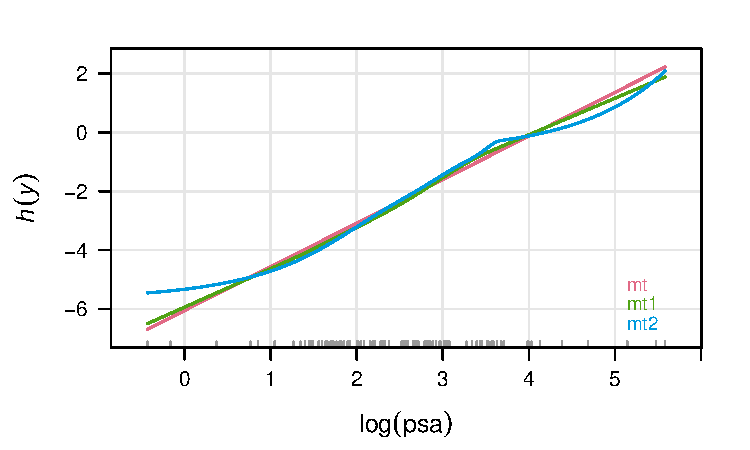
\includegraphics{BH_Linear5-1} 
\caption{Comparison of different choices for the baseline transformation of the
response (prostate-specific antigen concentration) in the \code{Prostate} data.
The original analysis prespecified a log-transformation of the response and then
assumed conditional normality on this scale. Hence the baseline transformation
of \code{mt} is of the form: $\h(\mathrm{lpsa}) = \eparm_1 + \eparm_2 \cdot
\mathrm{lpsa}$. Now, one can allow a more flexible transformation function in
$\log($\code{psa}$)$ to judge any deviations of $\h(\log(\mathrm{psa}))$ from
linearity, leading to a baseline transformation in terms of basis functions:
$\bern{7}(\log(\mathrm{psa}))^\top \parm$ in \code{mt1}. Lastly, instead of
presuming a log-transformation, one could estimate the baseline transformation
from the raw response (\code{psa}), \ie $\h(\mathrm{psa}) = \bern{11}
(\mathrm{psa})^\top \parm$ in \code{mt2}. In this case, a higher-order basis
expansion was chosen to account for the skewness of the raw response. Notably,
all three baseline transformations are fairly comparable. The basis expansion
in \code{psa} deviates from being log-linear towards the boundaries of the
response's support, as there are only a few observations.}
\label{fig:Prostate_trafos}
\end{figure}

\begin{table}
\centering
\begin{tabular}{lrrrrrrrrr}
\toprule
\multicolumn{1}{c}{\textbf{Model}} & \multicolumn{8}{c}{\textbf{Coefficient estimates}} & \multicolumn{1}{c}{\textbf{logLik}} \\
\cmidrule(l{3pt}r{3pt}){1-1} \cmidrule(l{3pt}r{3pt}){2-9} \cmidrule(l{3pt}r{3pt}){10-10}
  & lcavol & lweight & age & lbph & svi & lcp & gleason & pgg45 &  \\
\midrule
\code{mp} & 0.69 & 0.23 & -0.15 & 0.16 & 0.32 & -0.15 & 0.03 & 0.13 & -99.5\\
\code{mt} & 1.03 & 0.33 & -0.22 & 0.23 & 0.47 & -0.22 & 0.05 & 0.19 & -99.5\\
\code{mtp} & 1.03 & 0.33 & -0.22 & 0.23 & 0.47 & -0.22 & 0.05 & 0.19 & -339.9\\
\code{mt1} & 1.03 & 0.34 & -0.21 & 0.22 & 0.48 & -0.23 & 0.04 & 0.22 & -338.0\\
\code{mt2} & 0.97 & 0.32 & -0.19 & 0.22 & 0.48 & -0.21 & 0.07 & 0.21 & -343.5\\
\bottomrule
\end{tabular}
\caption{Comparison of the three transformation models on the \code{Prostate} data.
Coefficient estimates are shown for each model, together with the in-sample
log-likelihood in the last column. The first three models, \code{mp}, \code{mt}, and
\code{mtp} use a linear baseline transformation in \code{lpsa} and $\log($\code{psa}$)$,
respectively. The \code{mp} model was fit using \pkg{penalized} and gave the scaled
version of the regression coefficients in \code{mt}, but the same log-likelihood.
At the same time, \code{mt} and \code{mtp} differ only in their response variable
and its subsequent log-transformation in \code{mtp}, yielding the same coefficient
estimates but a different log-likelihood. Models \code{mt1} and \code{mt2} allow a
flexible basis expansion in $\log($\code{psa}$)$ and \code{psa}, respectively.
Model \code{mt1}, allowing for a flexible basis expansion in \code{lpsa}, fits the
data the best. However, the resulting coefficient estimates are similar for all
models.} \label{tab:prostatemods}
\end{table}


\subsection{Hyperparameter tuning} \label{sec:tuning}

This section features cross-validation, model-based optimization, and profiling functions
for hyperparameter tuning, whose appropriate values are highly problem-dependent
and hard to know in advance. \pkg{tramnet} implements naive grid search and model-based
optimization in the functions \cmd{cvl\_tramnet} and \cmd{tramnet\_mbo}, respectively.
In the framework of regularized transformation models, it is very natural to choose
the out-of-sample log-likelihood as the objective function because
the notion of a mean square loss does not make sense for survival, let alone
censored outcomes. The out-of-sample log-likelihood is, in fact, the log score,
which is a proper scoring rule \citep{Gneiting_Raftery_2007}.
\begin{example}
R> m0 <- BoxCox(lpsa ~ 1, data = Prostate, order = 7, extrapolate = TRUE)
R> mt <- tramnet(m01, x = x, alpha = 1, lambda = 0)
\end{example}
\pkg{tramnet} offers cross-validation in \cmd{cvl\_tramnet}, comparable to the
\cmd{optL1}, and \cmd{optL2} functions in \pkg{penalized}, which takes a sequence
of values for $\lambda$ and $\alpha$ and performs a simple --~and arguably slow~--
grid search. Per default, it computes 2-fold cross-validation. The user is encouraged,
however, to judge the resulting bias-variance trade-off accordingly.
\begin{example}
R> lambdas <- c(0, 10^seq(-4, log10(15), length.out = 4))
R> cvlt <- cvl_tramnet(object = mt, fold = 2, lambda = lambdas, alpha = 1)
\end{example}
In order to compare cross-validation across multiple packages and functions, it
is also possible to supply the folds for each row in the design matrix as a
numeric vector, as for example returned by \cmd{penalized::optL1}.
\begin{example}
R> pen_cvl <- optL1(response = lpsa, penalized = x, lambda2 = 0, data = Prostate,
+                   fold = 2)
R> cvlt <- cvl_tramnet(object = mt, lambda = lambdas, alpha = 1,
+                      folds = pen_cvl$fold)
\end{example}
The resulting object is of class \cls{cvl\_tramnet} and contains a table for the
cross-validated log-likelihoods for each fold and the sum thereof, the `optimal'
tuning parameter constellation, which resulted in the largest cross-validated
log-likelihood, tables for the cross-validated regularization paths, the
folds and lastly the full fit based on the `optimal' tuning parameters. Additionally,
the resulting object can be used to visualize the log-likelihood and coefficient
trajectories. These trajectories highly depend on the chosen folds, and the user
is referred to the full profiling functions discussed in Section~\nameref{subsec:prof}.

\subsubsection{Model-based optimization} \label{subsec:prostatembo}

In contrast to naive grid search, model-based optimization comprises more
elegant methods for hyperparameter tuning. \pkg{tramnet} offers the \cmd{mbo\_tramnet}
and \cmd{mbo\_recommended} functions. The former implements Kriging-based hyperparameter
tuning for the elastic net, the Lasso, and ridge regression. \cmd{mbo\_tramnet}
takes a \cls{tramnet} object as input and computes the cross-validated log-likelihood
based on the provided \code{fold} or \code{folds} argument. The initial design
is a random latin hypercube design with \code{n\_design} rows per parameter.
The number of sequential fits of the surrogate models is specified through
\code{n\_iter}, and the range of the tuning parameters can be specified by
\code{max/min} arguments. The default infill criterion is expected improvement.
However, \citet{mlrMBO} encourage the use of the lower confidence bound over
expected improvement, which can be achieved in \cmd{mbo\_tramnet} by specifying
\code{opt\_crit~=~makeMBOInfillCritCB()}. 10-fold cross-validation is used to compute
the objective function for the initial design and each iteration. The recommended
model is then extracted using \cmd{mbo\_recommended}.
\begin{example}
R> tmbo <- mbo_tramnet(mt, obj_type = "elnet", fold = 10)
R> mtmbo <- mbo_recommended(tmbo, m0, x)
\end{example}

Unlike in the previous section, one can directly optimize the tuning parameters
in an elastic net problem instead of optimizing over one hyperparameter at a time
or having to specify Lasso or ridge regression \emph{a priori}. The output of
\cmd{mbo\_tramnet} is quite verbose and can be shortened by using the helper
function \cmd{print\_mbo}.
\begin{example}
R> print_mbo(tmbo)

## Recommended parameters:
## lmb=1.04e-05; alp=0.751 
## Objective: y = 710 
\end{example}
Interpreting the output, model-based optimization suggests an unpenalized model
with $\alpha = 0.75$ and $\lambda = 0$.
This result stresses the advantages of model-based optimization over naive or random
grid search in terms of complexity and computational efficiency. In the end, the
proposed model is unpenalized and thus does not introduce sparsity in the regression
coefficients.
\begin{example}
R> coef(mtmbo)

## lcavol lweight     age    lbph     svi     lcp gleason   pgg45 
## 1.0312  0.3380 -0.2068  0.2198  0.4801 -0.2329  0.0437  0.2157 

R> summary(mtmbo)$sparsity
## [1] "8 regression coefficients, 8 of which are non-zero"
\end{example}

\subsubsection{Regularization paths} \label{subsec:prof}

As discussed before, it may be useful to inspect the full regularization paths
over the tuning parameters $\lambda$ and $\alpha$. Akin to the functions \cmd{profL1}
and \cmd{profL2} in package \pkg{penalized}, \pkg{tramnet} offers \cmd{prof\_lambda}
and \cmd{prof\_alpha}. Since these functions take a fitted model of class
\cls{tramnet} as input, which is internally updated, it is crucial to correctly
specify the other tuning parameter in the model fitting step. In the example to
come, \code{mt} was fit using $\alpha = 1$ and $\lambda = 0$, resulting in a
Lasso penalty only when profiling over $\lambda$. The resulting profile is depicted
in Figure~\ref{fig:prof}.
\begin{example}
R> pfl <- prof_lambda(mt)
\end{example}
\cmd{prof\_lambda} takes \code{min\_lambda}, \code{max\_lambda}, and \code{nprof}
as arguments and internally generates an equi-spaced sequence from \code{min\_lambda}
to \code{max\_lambda} on the log scale of length \code{nprof}. By default, this
sequence ranges from $0$ to $15$ and is of length $5$.
\begin{example}
R> plot_path(pfl, plot_logLik = FALSE, las = 1, col = coll)
\end{example}

\begin{figure}
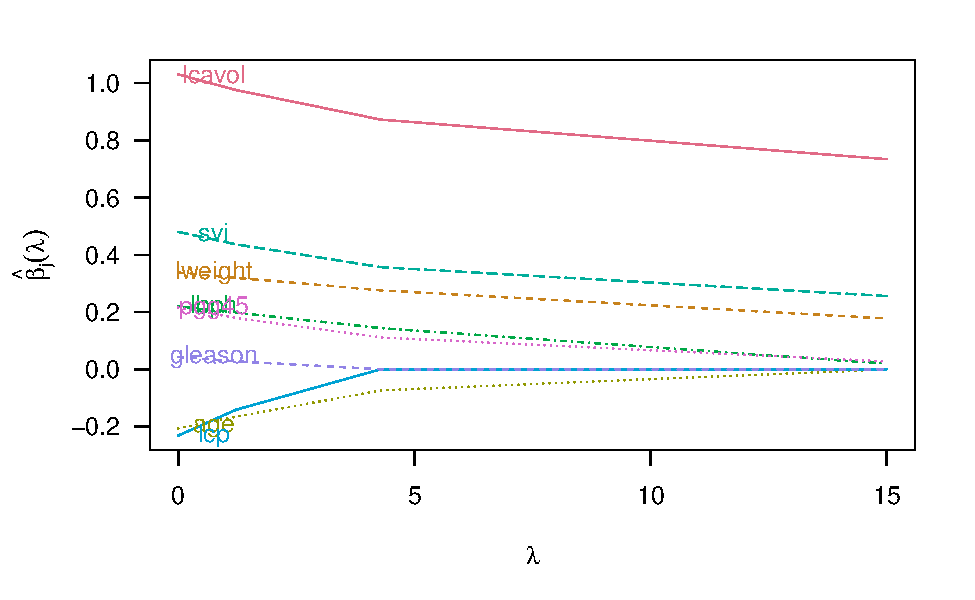
\includegraphics[width=1\textwidth]{profiling_plot-1} 
\caption{Full regularization paths for the tuning parameter $\lambda$ using the
default values of \cmd{plot\_path}.}
\label{fig:prof}
\end{figure}

\subsection{Additional constraints} \label{subsec:otherconstr}

In some applications, the specification of additional constraints on the shift
parameters $\shiftparm$ are of interest. Most commonly, either positivity or
negativity for some or all regression coefficients is aimed at. In \pkg{tramnet},
additional inequality constraints can be specified via the \code{constraints} argument,
which are internally handled as \code{constraints[[1]] \%*\% beta $>$ constraints[[2]]}. 
Hence, to specify the constraint of strictly positive regression coefficients, 
one would supply an identity matrix of dimension $p$ for the left-hand side and
the zero $p$-vector for the right-hand side, as done in the following example.
\begin{example}
R> m0 <- BoxCox(lpsa ~ 1, data = Prostate, extrapolate = TRUE)
R> mt <- tramnet(m0, x, alpha = 0, lambda = 0, constraints = list(diag(8),
+                                                                 rep(0, 8)))
R> coef(mt)

## lcavol lweight    lbph     svi gleason   pgg45 
## 0.9111  0.2996  0.1684  0.3969  0.0133  0.1125 
\end{example}
The coefficients with a negative sign in the model without additional positivity
constraints now shrink to zero, with the other coefficient estimates changing
as well.
\begin{example}
R> summary(mt)$sparsity

## [1] "8 regression coefficients, 6 of which are non-zero"
\end{example}
One can compare this model to the implementation in \pkg{tram}, where it is also
possible to specify linear inequality constraints on the regression coefficients
$\shiftparm$. Here, it is sufficient to specify
\code{constraints = c("age >= 0", "lcp >= 0")}
for the two non-positive coefficient estimates.
\begin{example}
R> m <- BoxCox(lpsa ~ . - psa, data = Prostate, extrapolate = TRUE,
+              constraints = c("age >= 0", "lcp >= 0"))
R> max(abs(coef(m) - coef(mt, tol = 0)))

## [1] 1.28e-05
\end{example}
Indeed, both optimizers arrive at virtually the same coefficient estimates.

%%%%%%%%%%%%%%%%%%%%%%%%%%%%%%%%%%%%%%%%%%%%%%%%%%%%%%%%%%%%%%%%%%%%%%%%%%%%%%%%
\section{\texorpdfstring{\code{S3}}{S3} Methods} \label{sec:methods}
%-------------------------------------------------------------------------------

Building on the \code{S3} infrastructure of the packages \CRANpkg{mlt} and \pkg{tram},
this package provides corresponding methods for the following generics: \cmd{coef},
\cmd{logLik}, \cmd{plot}, \cmd{predict}, \cmd{simulate}, and \cmd{residuals}.
The methods' additional \cls{tramnet}-specific arguments will be briefly discussed
in this section.

\cmd{coef.tramnet} suppresses the baseline transformation's coefficient estimates
$\hat\parm$ by default and considers shift parameter estimates $\hat\shiftparm$
below $10^{-6}$ as $0$ to stress the selected variables only.
This threshold can be controlled by the \code{tol} argument.
Hence, \code{coef(mt, with\_baseline = TRUE, tol = 0)} returns all coefficients.
\begin{example}
R> coef(mtmbo, with_baseline = TRUE, tol = 0)

## Bs1(lpsa) Bs2(lpsa) Bs3(lpsa) Bs4(lpsa) Bs5(lpsa) Bs6(lpsa) Bs7(lpsa) 
##   -1.9775   -1.5055   -1.0335   -0.2778   -0.2778    1.0723    1.5150 
## Bs8(lpsa)    lcavol   lweight       age      lbph       svi       lcp 
##    1.9576    1.0312    0.3380   -0.2068    0.2198    0.4801   -0.2329 
## gleason     pgg45 
##    0.0437    0.2157 
\end{example}
The \cmd{logLik.tramnet} method allows the log-likelihoods re-computation under
new data (\ie out-of-sample) and different coefficients (\code{parm}) and weights
(\code{w}), as illustrated below.
\begin{example}
R> logLik(mtmbo)

## 'log Lik.' -97.7 (df=NA)

R> cfx <- coef(mtmbo, with_baseline = TRUE, tol = 0)
R> cfx[5:8] <- 0.5
R> logLik(mtmbo, parm = cfx)

## 'log Lik.' -561 (df=NA)

R> logLik(mtmbo, newdata = Prostate[1:10,])

## 'log Lik.' -14.3 (df=NA)

R> logLik(mtmbo, w = runif(n = nrow(mtmbo$x)))

## 'log Lik.' -41.8 (df=NA)
\end{example}
In the spirit of \pkg{mlt}'s plotting methods for classes \cls{mlt} and \cls{ctm},
\cmd{plot.tramnet} offers diverse plotting options for objects of class \cls{tramnet}.
The specification of new data and the type of plot is illustrated in the following code
chunk and Figure~\ref{fig:plot}.
\begin{example}
R> par(mfrow = c(3, 2)); K <- 1e3
R> plot(mtmbo, type = "distribution", K = K, main = "A") # A, default
R> plot(mtmbo, type = "survivor", K = K, main = "B") # B
R> plot(mtmbo, type = "trafo", K = K, main = "C") # C
R> plot(mtmbo, type = "density", K = K, main = "D") # D
R> plot(mtmbo, type = "hazard", K = K, main = "E") # E
R> plot(mtmbo, type = "trafo", newdata = Prostate[1, ], col = 1, K = K, main = "F") # F
\end{example}

\begin{figure}[!ht]
\centering 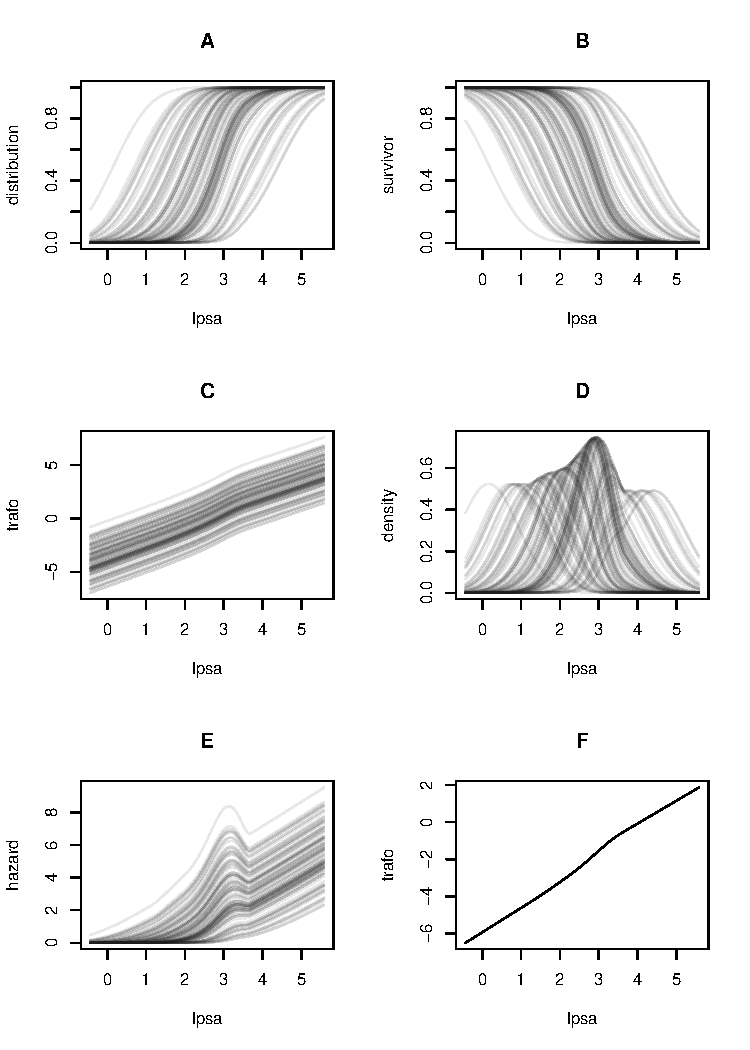
\includegraphics{plot_method_fig-1} 
\caption{Illustration of \cmd{plot.tramnet}'s versatility in visualizing the
response's estimated conditional distribution on various scales, including cdf,
survivor, transformation scale and pdf. Note that, by default, the plot is produced
for each row in the design matrix. In unstratified linear transformation models,
this leads to shifted versions of the same curve on the transformation function's
scale.
A: Estimated conditional distribution function for every observation.
B: Estimated conditional survivor function for every observation. The conditional
survivor function is defined as $S(\ry \given \rx) = 1 - \pY(\ry \given \rx)$.
C: Conditional most likely transformation for every observation. Note that every conditional
transformation function is a shifted version of the same curve.
D: The conditional density for every observation can be calculated using
$\dY(\ry \given \rx) = F'(\basisy(\ry)^\top\parm - \rx^\top\shiftparm)\basisy'
  (\ry)^\top\parm$.
E: A distribution function is fully characterized by its hazard function
$\lambda(\ry \given \rx) = \dY(\ry \given \rx) / S(\ry \given \rx)$, which is depicted
in this panel.
F: The \code{newdata} argument can be used to plot the predicted most likely transformation
for the provided data, in this case, the first row of the \code{Prostate} data.}
\label{fig:plot}
\end{figure}

The \cmd{predict.tramnet} method works in the same way as \cmd{predict.mlt} and
as such supports the types \code{trafo, distribution, survivor, density, logdensity,
hazard, loghazard, cumhazard}, and \code{quantile}. For \code{type = "quantile"},
the corresponding probabilities (\code{prob}) have to be supplied as an argument
to evaluate the quantile function.
\begin{example}
R> predict(mtmbo, type = "quantile", prob = 0.2, newdata = Prostate[1:5,])
       
## prob    [,1] [,2] [,3] [,4] [,5]
##     0.2  3.4 3.55 3.74 3.72 2.68
\end{example}
Another method offered by this package implements parametric bootstrap-based
sampling. In particular, \cmd{simulate.tramnet} calls the \cmd{simulate.ctm}
function after converting the \cls{tramnet} object to a \cls{ctm} object.
\begin{example}
R> simulate(mtmbo, nsim = 1, newdata = Prostate[1:5,], seed = 1)

## [1] 3.56 3.97 4.57 5.48 2.69
\end{example}
Lastly, \cmd{residuals.tramnet} computes the generalized residual $r$ defined as
the score contribution for sample $i$ with respect to a newly introduced intercept
parameter $\gamma$, which is restricted to be zero. In particular,

\begin{align*}
  r = \frac{\partial \ell\left(\parm,\shiftparm,\gamma;\ry, \rs, \rx\right)}{\partial
    \gamma} \bigg\rvert_{\gamma = 0}
\end{align*}
yields the generalized residual with respect to $\gamma$ for the model

\begin{align*}
  \pY(\ry \given \rs, \rx) = F\left(\h(y \mid \rs) - \rx^\top \shiftparm - \gamma \right).
\end{align*}
\begin{example}
R> residuals(mtmbo)[1:5]

## [1] -6.50 -6.36 -6.60 -6.57 -4.17
\end{example}
In residual analysis and boosting, it is common practice to check for associations
between residuals and covariates that are not included in the model.
In the prostate cancer example, one could investigate whether the variables \code{age}
and \code{lcp} should be included in the model. To illustrate this particular case,
a nonparametric \cmd{independence\_test} from package \CRANpkg{coin} can be used \citep{coinjss}.
First, the uncoditional transformation model \code{m0} is fitted. Afterward, the tramnet
models excluding \code{age} and \code{lcp} are estimated, and their residuals
extracted using the \cmd{residuals.tramnet} method. Lastly, an independence test
using a maximum statistic (\code{teststat~=~"max"}) and a Monte Carlo-based
approximation of the null distribution based on resampling $10^6$ times
(\code{distribution~=~approximate(1e6)}) yields the results printed below.
\begin{example}
R> library("coin")
R> m0 <- BoxCox(lpsa ~ 1, data = Prostate, extrapolate = TRUE)
R> x_no_age_lcp <- x[, !colnames(x) %in% c("age", "lcp")]
R> mt_no_age_lcp <- tramnet(m0, x_no_age_lcp, alpha = 0, lambda = 0)
R> r <- residuals(mt_no_age_lcp)
R> it <- independence_test(r ~ age + lcp, data = Prostate,
+                          teststat = "max", distribution = approximate(1e6))
R> pvalue(it, "single-step")

## age  0.023748
## lcp <0.000001
\end{example}
Because there is substantial evidence against the independence of the models' residuals 
to either \code{lcp} or \code{age}, we can conclude that it is
worthwhile to include \code{age} and \code{lcp} in the model.
Packages \CRANpkg{trtf} \citep{pkg:trtf} and \CRANpkg{tbm} \citep{hothorn2019tbm,pkg:tbm}
make use of this definition of a residual for estimating and boosting transformation models,
trees, and random forests. For more theoretical insight, the reader is referred to
the above mentioned publications.

%%%%%%%%%%%%%%%%%%%%%%%%%%%%%%%%%%%%%%%%%%%%%%%%%%%%%%%%%%%%%%%%%%%%%%%%%%%%%%%%
\newpage
\bibliography{kook-hothorn}

\address{Lucas Kook, Torsten Hothorn\\
  Institut f\"ur Epidemiologie, Biostatistik und Pr\"avention \\
  Universit\"at Z\"urich \\
  Hirschengraben 84, CH-8001 Z\"urich\\
  Switzerland\\
  \email{lucasheinrich.kook@uzh.ch}, \email{Torsten.Hothorn@R-project.org}}
